\chapter{準備}\label{chapter:Prepare}
\section{章の概略}\label{section:Outline}
この章では準備としてペンシルパズルに関わる用語の定義を行う. ただし, ペンシルパズルとは「サイズ$m\times n$の平面グリッドを与えたとき, パズルルールに定められた条件と, その解答ステップにおいて明らかになっている解から格子点, 細胞, 辺のいずれかの未知情報に論理的推測から解を書き込み, 全ての格子点, 細胞, 辺がパズルルールに定められた条件を満たす完成盤面へと解く行為と, その問題やルールなどを一括りに呼ぶ概念」とし, 明確な定義は行わずあくまで概念として以下もペンシルパズルという用語を使用する. ただし, 格子点, 細胞, 辺というのは\cref{fig:Board}で与える図中の名前とそれぞれ対応させるものとする.
ペンシルパズルは, 例としてナンバープレイス(\cref{fig:SamplePuzzle})などが与えられる.
\cref{section:WordDefinition}ではペンシルパズルで与えられる盤面と, それに付随する用語を定義する.
\cref{section:MathematicalDefinition}ではペンシルパズルにおける, 諸概念の数学的な定義を行う.
\cref{section:RelationDefinition}では\cref{section:MathematicalDefinition}で定義する変数同士の関係性についての定義を行う.
\cref{section:GraphDefinition}ではペンシルパズルにおいて考えられるグラフという概念の定義を行う.

\section{用語の定義}\label{section:WordDefinition}
この節ではペンシルパズルにおける用語を定義する. ただし, ペンシルパズルとは「サイズ$m\times n$の平面グリッドを与えたとき, 格子点, 細胞, 辺のいずれかの未知情報に対し, パズルルールに定められた条件とその解答ステップにおいて明らかになっている既知情報から一意に定まる解を書き込み, 全ての格子点, 細胞, 辺がパズルルールに定められた条件を満たす完成盤面へと解く行為と, その問題やルールなどを一括りに呼ぶ概念」とし, 明確な定義は行わずあくまで概念として以下もペンシルパズルという用語を使用する. ただし, 格子点, 細胞, 辺は\cref{fig:Board}で与える図中の名前とそれぞれ対応させるものとし, ある解答ステップにおける既知情報とはあるパズルの問題があったときの初期状態と, それまでの解答ステップにより得られた解のことを指すものとする. ペンシルパズルは, 例としてナンバープレイス(\cref{fig:SamplePuzzle})などが与えられる.

以下の説明のために盤面, 完成盤面, 未完成盤面を定義する. \cref{fig:Board}で与えたようなグリッドに対し, 各格子点, 細胞, 辺に対応する解が存在するものを総称して\textgt{盤面}と定義する. しかし, その解が未知, 既知に関わらず盤面と呼ぶ. ただし解とはペンシルパズルにおいて格子点, 細胞, 辺に対して写像で送った際に数値や, 変数のことである. \cref{fig:SamplePuzzle}に与えたパズルでは, 左上端の細胞の解が2に対応し, 右下端の細胞の解は未知である(既知の場合3).
また, 全ての格子点, 細胞, 辺の解がパズルルールに定められた条件を満たしている盤面のことを\textgt{完成盤面}と定義する. さらに任意の格子点, 細胞, 辺の解が未知であるものが存在する盤面の中で, 解を既知にしたときに対応する完成盤面がただ一つしかない盤面を\textgt{未完成盤面}と定義する. 未完成盤面と完成盤面の例として\cref{fig:SamplePuzzle}を与える. 図中左が未完成盤面, 図中右が完成盤面である.

上の記述より, 一つの完成盤面には複数の未完成盤面が対応する(一つの操作(未知情報に解を書き込む)を課した未完成盤面もまた未完成盤面. ).このとき, その複数の未完成盤面と, 完成盤面の集合全体をパズルルールの\textgt{問題}と定義する.

\begin{clearpagefigure}

  
\includegraphics[width=8cm,clip]{fig/board.png}
  \caption{}
  \label{fig:Board}
\end{clearpagefigure}

\begin{clearpagefigure}
  
\includegraphics[width=8cm,clip]{fig/samplePuzzle.png}
  \caption{}
  \label{fig:SamplePuzzle}
\end{clearpagefigure}

\section{盤面上の情報に関する概念の数学的定義}\label{section:MathematicalDefinition}
この節ではペンシルパズルにおける盤面上の情報に関する各概念を数学的に定義する. ここで定義するものは全て直感的な定義と違わないように行う.
平面グリッドを与えたとき, ペンシルパズルの盤面には左上から各格子点に対し座標$(i,j)$を割り振ることができる(\cref{fig:Coordinate}). そうしたとき, グリッドにおける格子点, 細胞, 辺に対して\cref{fig:VariableAtBoard}で表されるように変数を与えることができる.
これをそれぞれ数学的に格子点$p(i,j)$, 細胞$c(i,j)$, 横辺$h(i,j)$, 縦辺$v(i,j)$として定義する.

\begin{clearpagefigure}
  
\includegraphics[width=8cm,clip]{fig/coordinate.png}
  \caption{}
  \label{fig:Coordinate}
\end{clearpagefigure}

\begin{definition}[格子点$p(i,j)$, 細胞$c(i,j)$, 横辺$h(i,j)$, 縦辺$v(i,j)$]\label{definition:VariableAtBoard}
  \textgt{格子点}$p(i,j)$($(i,j)\in \mathbb{Z}^2$)を
  \begin{equation*}
    p(i,j)\coloneqq \{(i,j)\} \quad (1\leq i \leq n, 1\leq j \leq n)
  \end{equation*}
  と定義する.

  以下同様に\textgt{細胞}$c(i,j)$, \textgt{横辺}$h(i,j)$, \textgt{縦辺}$v(i,j)$を
  \begin{gather*}
    c(i,j)\coloneqq  \{(i,j), (i,j+1), (i+1,j), (i+1,j+1)\}  (1\leq i \leq n-1, 1\leq j \leq n-1)  \\
    h(i,j)\coloneqq  \{(i,j), (i,j+1)\}                      (1\leq i \leq n-1, 1\leq j \leq n)    \\
    v(i,j)\coloneqq  \{(i,j), (i+1,j)\}                      (1\leq i \leq n, 1\leq j \leq n-1)
  \end{gather*}
  と定義する.

  ただし, $h(i,j),v(i,j)$の詳細に興味がない場合は, 任意の辺という意味で辺$e(i,j,y)$を
  \begin{equation*}
    e(i,j,y) \coloneqq \{h(1,1),h(1,2),...,h(n-1,n),v(1,1),v(1,2),...,v(n,n-1)\}\ni \forall x \quad (y \in \{h,v\})
  \end{equation*}
  と定義する.
  ただし, $y=h$のとき$e(i,j,h)$は縦辺, $y=v$のとき$e(i,j,v)$は横辺を指すものとする. $(i,j)$の範囲はyによって指定されるそれぞれの変数によって定義されるものとする($y=h$のときは$1\leq i \leq n-1,1\leq j \leq n$).

  また, 格子点, 細胞, 辺の集合の詳細そのものに興味がない場合は任意の格子点, 細胞, 辺という意味で$\lambda(i,j,y)$を
  \begin{equation*}
    \lambda(i,j,y) \coloneqq \{p(i,j),c(i,j),h(i,j),v(i,j)\}\ni \forall x \quad (y \in \{p,c,h,v\})
  \end{equation*}
  と定義する.ただし, $y=p$のときは$\lambda(i,j,p)$は格子点, $y=c$のときは$\lambda(i,j,c)$は細胞, $y=h$のときは$\lambda(i,j,h)$は縦辺, $y=v$のときは$\lambda(i,j,v)$は横辺を指すものとする. $(i,j)$の範囲はyによって指定されるそれぞれの変数によって定義されるものとする($y=p$のときは$1\leq i \leq n,1\leq j \leq n$).
\end{definition}
これら添え字付きの変数を改めて格子点, 細胞, 辺と呼び, これらをまとめた総称として\textgt{盤面上の変数}と呼ぶこととする.

\begin{clearpagefigure}
  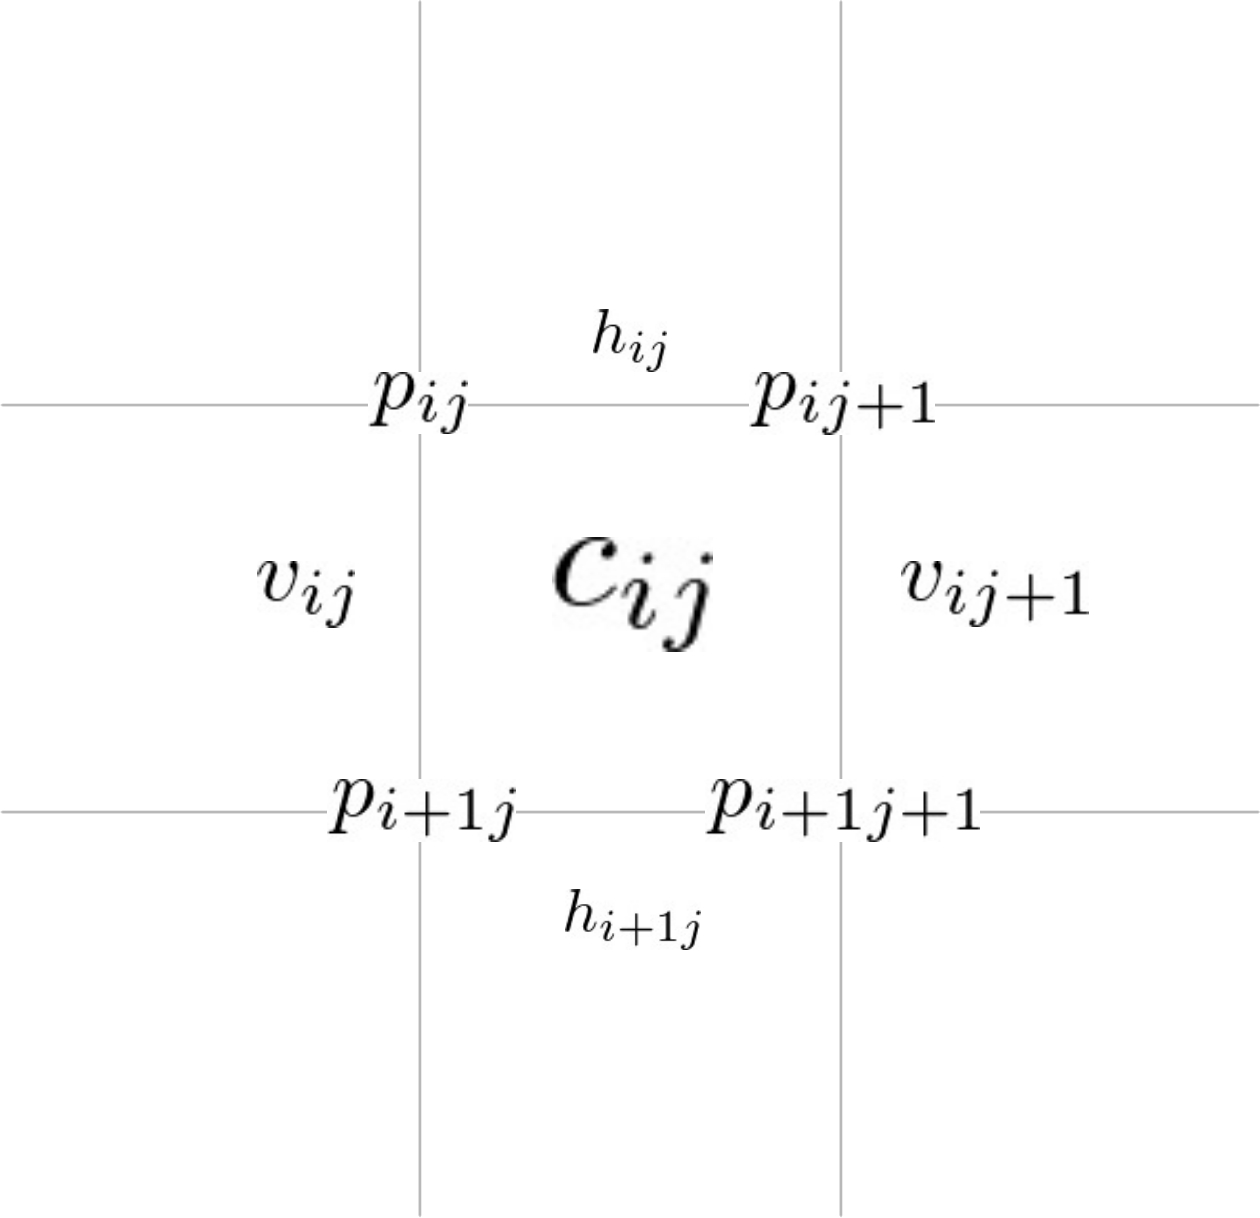
\includegraphics[width=8cm,clip]{fig/define.png}
  \caption{}
  \label{fig:VariableAtBoard}
\end{clearpagefigure}

ペンシルパズルにおいて, ソルバーは盤面上の変数に対して解を書き込むことが前提であった(\cref{section:Outline}).解とは, 盤面上の変数に対応して与えられる数値や, 変数のことを指すものとする.
そのため, パズルルールを定義するためには, 解がどのような集合の元に含まれるかを定義する必要がある. そのために以下で\textit{codomain}という用語を用いて解集合を定義する.

\begin{definition}[\textit{codomain}]\label{definition:Codomain}
  盤面上の変数に対し一対一に対応する解が含まれる集合のことを\textbf{\textit{codomain}}と定義する. 格子点, 細胞, 辺の\textit{codomain}を表す集合として$\mathbb{P},\mathbb{C},\mathbb{H},\mathbb{V}$を用いる. $\mathbb{H},\mathbb{V}$の\textit{codomain}が一致している場合にはまとめて$\mathbb{E}$と記述する. \textit{codomain}の詳細に興味がなく, \textit{codomain}全体を考えるときにはそれら集合を含意するものとして$\Lambda$を使用する.
\end{definition}

ここで, 盤面上の変数に対してそれぞれ解として具体的な値(1や3などの数値, あるいは$x_1$などの記号)が対応するがその解は列をなしていて同一の値が含んだ列となることがある.
よって\textit{codomain}と解の列は同一視できないことに注意する. また, パズルルールによっては格子点, 細胞, 辺に解を与えられない場合があり, そのときに限っては\textit{codomain}は$\emptyset$と記述し, 盤面上の変数に対応する解が存在しないことを表すこととする.以下に既存のパズルルールのスリザーリンクを例として用いる. ただし, スリザーリンクのパズルルールは以下のものである. \cite{web:SlitherLink}

\begin{enumerate}
  \item 点と点の間にタテヨコに線を引き, 全体で1つの輪っかを作りましょう.
  \item 4つの点で作られた正方形の中にある数字は, その正方形の辺に引く線の数を表しています. 数字のない正方形には, 何本の線を引くかわかりません.
  \item 線を交差させたり, 枝分かれさせたりしてはいけません.
\end{enumerate}

\begin{clearpagefigure}
  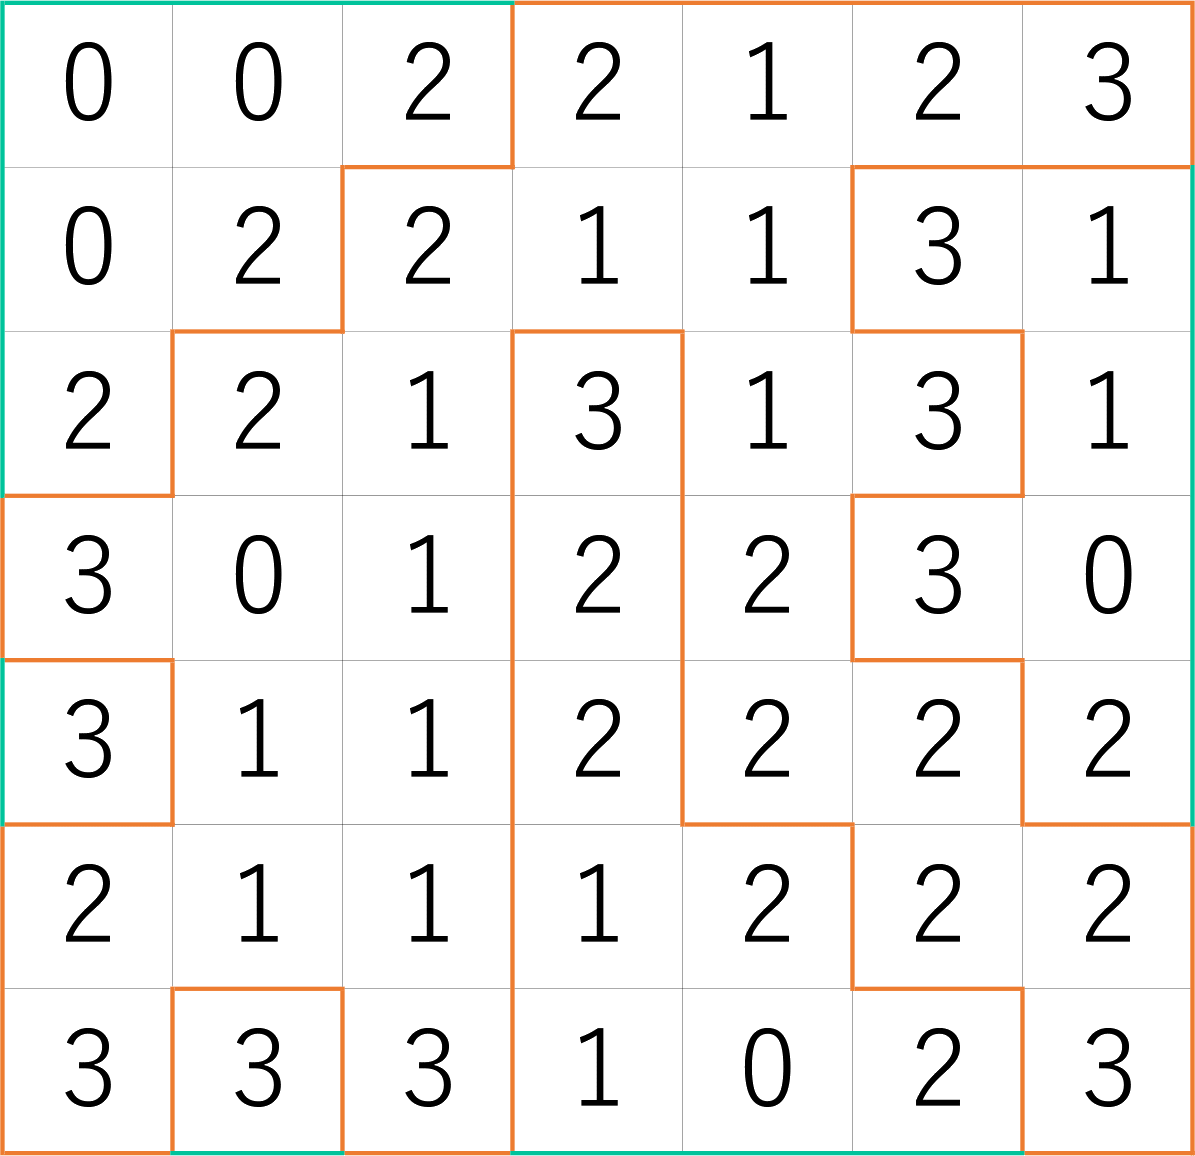
\includegraphics[width=5cm]{fig/slitherlink.png}
  \caption{スリザーリンクの完成盤面}
\end{clearpagefigure}

\begin{example}[スリザーリンクの\textit{codomain}]\label{example:SlitherLinkCodomain}
  スリザーリンクにおいては, \textit{codomain}は以下のように表すことができる. しかし辺が「書かれている」時は1,「書かれていない」時は0に対応させるものとする.
  \begin{gather*}
    \mathbb{P}  =  \emptyset     \\
    \mathbb{C}  =  \{0,1,2,3,4\} \\
    \mathbb{E}  =  \{0,1\}
  \end{gather*}
\end{example}
以上のように\textit{codomain}を考えることにより, 盤面上の変数が含まれる各集合から, \textit{codomain}に送る写像を考えることができる.
\begin{definition}[写像$\bm{p}$, $\bm{c}$, $\bm{h}$, $\bm{v}$]\label{definition:Mapping}
  格子点$p(i,j)$を過不足なくふくむ集合$\{p(i,j)\}$から$\mathbb{P}$に送る写像$\bm{p}$を
  \begin{equation*}
    \begin{array}{rccc}
      \bm{p}\colon & \{p(i,j)\} & \longrightarrow & \mathbb{P} \\
                   & p(i,j)     & \longmapsto     & p_{i,j}
    \end{array}
  \end{equation*}
  と定義する.
  以下同様に$\bm{c}$, $\bm{h}$, $\bm{v}$を

  \begin{equation*}
    \begin{array}{rccc}
      \bm{c}\colon & \{c(i,j)\} & \longrightarrow & \mathbb{C} \\
                   & c(i,j)     & \longmapsto     & c_{i,j}
    \end{array}
  \end{equation*}
  \begin{equation*}
    \begin{array}{rccc}
      \bm{h}\colon & \{h(i,j)\} & \longrightarrow & \mathbb{H} \\
                   & h(i,j)     & \longmapsto     & h_{i,j}
    \end{array}
  \end{equation*}
  \begin{equation*}
    \begin{array}{rccc}
      \bm{v}\colon & \{v(i,j)\} & \longrightarrow & \mathbb{V} \\
                   & v(i,j)     & \longmapsto     & v_{i,j}
    \end{array}
  \end{equation*}
  と定義する.

  ただし, $\bm{h},\bm{v}$の詳細に興味がない場合は, 同様に
  \begin{equation*}
    \begin{array}{rccc}
      \bm{e}\colon & \{e(i,j,y)\} & \longrightarrow & \mathbb{E} \\
                   & e(i,j,y)     & \longmapsto     & e_{i,j,y}
    \end{array}
  \end{equation*}
  と記述し, 上記の写像の詳細に興味がない場合それらの写像全てを含意するものとして$\bm{\lambda}$を用いて
  \begin{equation*}
    \begin{array}{rccc}
      \bm{\lambda}\colon & \{\lambda(i,j,y)\} & \longrightarrow & \Lambda         \\
                         & \lambda(i,j,y)     & \longmapsto     & \lambda_{i,j,y}
    \end{array}
  \end{equation*}
  と記述する.
\end{definition}
集合論の用語を用いると, 解の列$\{\lambda_{1,1,y_{(1,1)}}, \lambda_{1,2,y_{(1,2)}},...\}$と写像$\bm{\lambda}\colon \{\lambda(i,j,y)\} \longrightarrow \Lambda$の間には$\bm{\lambda}(\lambda(i,j,y))=\lambda_{i,j,y}$という自然な一対一対応が存在する.
ここで$\{\lambda_{i,j,y}\}$は$\{\lambda_{1,1,y_{(1,1)}}, \lambda_{1,2,y_{(1,2)}},...\}$であり, 写像$\bm{\lambda}$は$\{\lambda(i,j,y)\}$によって添え字付けられた族である. またこのとき, $\{\lambda(i,j,y)\}$は添字集合で, $\lambda(i,j,y)$はこの写像の添字である.

盤面上の変数とその解(\textit{codomain}の元)の対応は(\cref{definition:Mapping})のように添字によってラベル付けされ, 解同士の関係は(\cref{definition:Codomain})直後で記述したように実際に取る値の如何に関わらず別物として扱う.
盤面上の変数と, その解(\cref{definition:Mapping})との対応が全て分かっているとき, 写像はそれらの取る値を全て列として記述すれば$\bm{\lambda}\Leftrightarrow \{\lambda_{i,j,y}\}$と同一視することができる.

このような種々の定義を導入することにより, $\mathbb{P},\mathbb{C},\mathbb{E}$を与えたとき任意の盤面は
\begin{equation}\label{equation:U}
  U=\Bigl\{\{\bm{p},\bm{c},\bm{e}\}_x\Bigr\}=\biggl\{\Bigl\{\{p_{i,j}\}_x,\{c_{i,j}\}_x,\{e_{i,j,y}\}_x\Bigr\}_x\biggr\} \quad (1\leq x \leq |U|)
\end{equation}
なる集合の一つの元と言うことが出来る.
ただし, 写像$\bm{c}$などは各盤面においてただ一つ存在するものだから, ある具体的な盤面は$\{\bm{p},\bm{c},\bm{e}\}_x$, あるいは$\Bigl\{\{p_{i,j}\}_x,\{c_{i,j}\}_x,\{e_{i,j,y}\}_x\Bigr\}_x$と記述されることに注意する.
また, $\lambda(i,j,y)$が$\lambda_{i,j,y}$と一対一対応することより誤解の恐れがない場合は$\lambda(i,j,y) \in B  $,  $\lambda_{i,j,y}\in B $と記述する.
このときは$B$は集合として$B=\{\lambda(i,j,y)\}_x$を考え, $\lambda_{i,j,y}$も$\bm{\lambda}$によりBの元として扱うこととする.
ただし前と同様$\{\lambda(i,j,y)\}_x$とは$\{\lambda(1,1,y_{(1,1)}), \lambda_(1,2,y_{(1,2)}),...\}$を指すものとする.

ここで, ある問題を与えたとき完成盤面が満たしているべきパズルルールによって定められた条件は, そのまま\cref{equation:U}に条件として記述することができて, これを\textit{conditions}と定義する.
\begin{definition}[\textit{conditions}]\label{definition:Conditions}
  完成盤面において解が満たしているべき必要十分条件のことを\textbf{\textit{conditions}}と定義する.
\end{definition}
\textit{conditions}の具体例は\cref{section:GraphDefinition}で定義するグラフと\cref{definition:Function}で定義する関数を用いる必要があるため, 後の\cref{example:SlitherLinkConditions}で取り上げることとする.

上の\textit{conditions}を用いればあるパズルルールが存在したとき, 完成盤面全体の集合$X$は
\begin{equation}\label{equation:X}
  X=\biggl\{\Bigl\{\{p_{ij}\}_x,\{c_{ij}\}_x,\{e_{i,j,y}\}_x\Bigr\}_x\mid \rm{\textit{conditions}}\biggr\}
\end{equation}
と記述することができる. ベン図は\cref{fig:VennDiagram}のようになる.

\begin{clearpagefigure}
  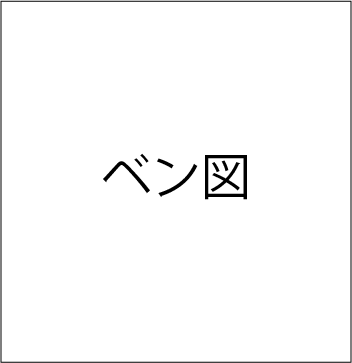
\includegraphics[width=8cm,clip]{fig/vennDiagram.png}
  \caption{}
  \label{fig:VennDiagram}
\end{clearpagefigure}

\cref{equation:X}で定義した完成盤面から問題へと派生させるために「ソルバーに隠す盤面上の変数の解」として\textit{HI(Hidden Information)}を定義する.
ただし, 「隠す」という言葉は\textit{codomain}から\textit{codomain}に\textit{null}を加えた集合$\Lambda'=\Lambda\cup \textit{null}$への写像$\phi\colon \Lambda \longrightarrow \Lambda'$を解の列に作用させることを意味することとする.
ただし, 解が未知であることを状態として\textbf{\textit{null}}と定義し, 盤面上の変数に対応する解が未知であるときに限り$p_{i,j}=\textit{null}$などとするとする.

ただし, パズルルールによっては解が未知である状態がソルバーに実際に示される数値あるいは変数が\textit{codomain}に含まれる場合があることに注意する. (スリザーリンク(\cref{example:SlitherLinkCodomain})においては$h_{i,j}, v_{i,j} = 0$のとき解が未知である, あるいは解として0を持つことがソルバーに同一の状態として伝えられる. )

\begin{definition}[\textit{HI(Hidden Information)}]\label{definition:HiddenInformation}
  ソルバーから隠す盤面上の変数の部分集合に対応する解の部分列を\textbf{\textit{HI(Hidden Information)}}と定義する.
  ただし, その部分集合はパズルルールによってそれが一意に定まるものではなく問題に依存するものとし, パズルルールでは$\{c_{i,j}\}$と$\{e_{i,j,y}\}$の部分列といったように隠す列及び部分列の情報のみを指定し, 詳細は指定しないものとする.
\end{definition}

\begin{example}[スリザーリンクの\textit{HI}]
  \begin{gather*}
    \{c_{i,j}\}の部分列 \\
    \{e_{i,j,y}\}
  \end{gather*}
\end{example}

完成盤面においては盤面上の変数と解が一対一に対応することにより, $\mathbb{E}$が要素として数値のみを持つ場合に限り新たに下記のような関数を導入することができる(\cref{fig:cross}, \cref{fig:cycle}).

\begin{definition}[\textit{cross}, \textit{cycle}]\label{definition:Function}
  \begin{gather*}
    \textit{cross}(p(i,j))\coloneqq h_{i,j-1}+v_{i-1,j}+h_{i,j}+v_{i,j} \\
    \textit{cycle}(c(i,j))\coloneqq h_{i,j}+v_{i,j}+h_{i+1,j}+v_{i,j+1}
  \end{gather*}
\end{definition}
\begin{clearpagefigure}
  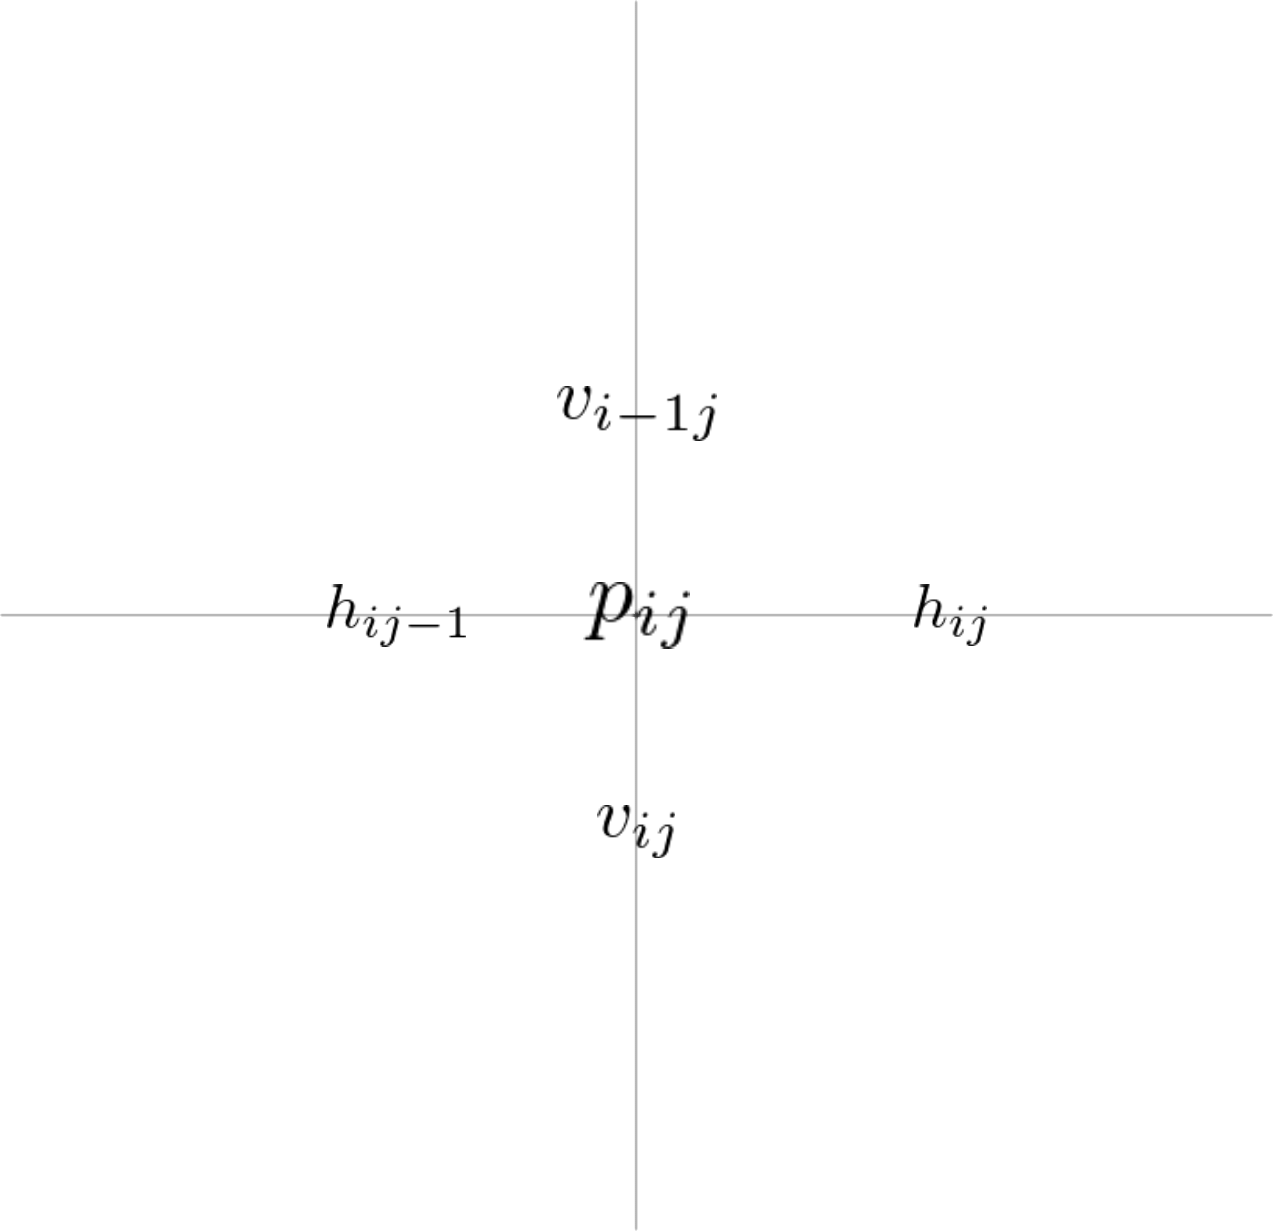
\includegraphics[width=5cm]{fig/cross.png}
  \caption{cross}
  \label{fig:cross}
\end{clearpagefigure}

\begin{clearpagefigure}
  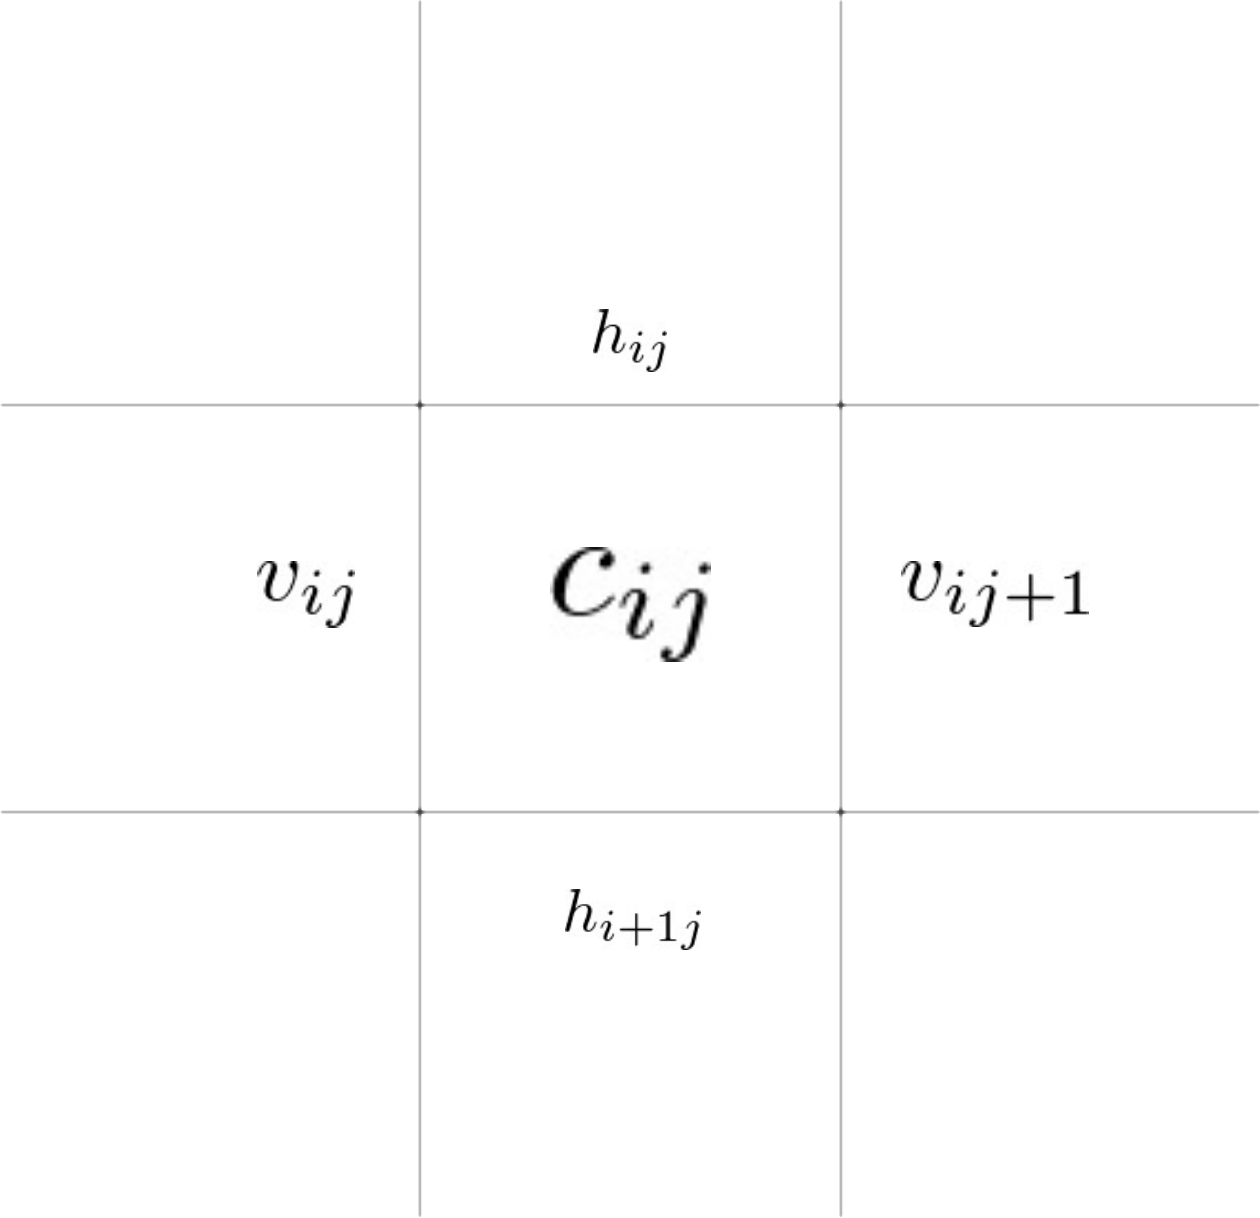
\includegraphics[width=5cm]{fig/cycle.png}
  \caption{cycle}
  \label{fig:cycle}
\end{clearpagefigure}

\section{盤面上の変数の関係性の定義}\label{section:RelationDefinition}

次に, \cref{section:MathematicalDefinition}で定義した盤面上の変数同士の関係性について定義を行う. ただし, ここでは完成盤面を仮定する.
まず, 連結と含有, 到達可能の定義を行う.
連結とは直感的に辺と辺が繋がっていることを表す用語とし, 含有とは盤面上の変数が集合として他の変数を含むこと, 到達可能とは離れた辺と辺へと向かう道が存在することを表す用語として導入する.

\begin{definition}[連結]\label{definition:Connection}
  $e(i,j,y)$と$e(i',j',y')$が\textbf{連結}であるとは, 以下が成立することで定義する.
  \begin{gather*}
    e_{i,j,y}=1, e_{i',j',y'}  =     1          \\
    e(i,j,y)\cup e(i',j',y')  \neq  \emptyset
  \end{gather*}
\end{definition}

\begin{definition}[含有]\label{definition:Contain}
  $e(i,j,y)$が$p(i',j')$を\textbf{含む(含有する)}とは以下が成立することで定義する.
  \begin{gather*}
    e_{i,j,y}=1               \\
    e(i,j,y)\supset p(i',j')
  \end{gather*}
  以下同様に, $c(i,j)$が$e(i',j',y')$を含む, $c(i,j)$が$p(i',j')$を含むことを以下が成立することでそれぞれ定義する.
  \begin{gather*}
    e_{i',j',y'}=1             \\
    c(i,j)\supset e(i',j',y')
  \end{gather*}
  \begin{gather*}
    c(i,j)\supset p(i',j')
  \end{gather*}
\end{definition}


\begin{definition}[到達可能]
  $e(i,j,y)$と連結な$e(i_1,j_1,y_1)$, $e(i_1,j_1,y_1)$と連結な$e(i_2,j_2,y_2),...,e(i_t,j_t,y_t)$と連結な$e(i',j',y')$のような集合$\{e(i_1,j_1,y_1),e(i_2,j_2,y_2),...,e(i_t,j_t,y_t)\}$がただ一つでも存在するとき, $e(i,j,y)$から$e(i',j',y')$に\textbf{辿ることが出来る(到達可能である)}と定義する. ただし, 自分自身は常に辿ることが出来るものとする.
\end{definition}

\begin{remark}
  $e(i,j,y)$から$e(i',j',y')$に辿ることが出来る(到達可能である)ときはいつでも$e(i',j',y')$から$e(i,j,y)$に辿ることが出来る.
\end{remark}

\begin{example}[連結, 含有, 到達可能]
  \cref{fig:SamplePuzzle}において, $h(4,1)$と$v(1,4)$は連結であり, $c(3,4)$は$v(4,4)$のみを含み, $h(3,8)$から$v(8,1)$へは辿ることが出来る.
\end{example}
以上の定義を用いることによって, 新たに「線」という概念を導入することができる.

\begin{definition}[線]\label{definition:Line}
  集合$L$の全ての要素から任意の2つの元を取り出したとき, いつでもそれらが互いに辿ることができるとき集合$L$を\textbf{線}であると定義する.
\end{definition}
この線はグラフ理論の用語を用いるたときの連結グラフとほとんど同義である. \cref{fig:SamplePuzzle}において, 集合$\{h(3,2),v(4,1),h(4,1),h(5,1)\}$は線である. この線も含有という関係性を定義することができて,
\begin{definition}[線の含有]
  線$L$が線$L'$を含むとは以下が成立することで定義する.
  \begin{equation*}
    L\supset L'
  \end{equation*}
  同様に線$L$が辺$e(i,j,y)$, 格子点$p(i,j)$が含むことを以下が成立することでそれぞれ定義する.
  \begin{equation*}
    L\supset  e(i,j,y) \\
  \end{equation*}
  \begin{equation*}
    L\ni \exists e(i,j,y) \quad \mbox{s.t. $e(i,j,y)$が$p(i,j)$を含む}
  \end{equation*}
\end{definition}

\section{グラフ}\label{section:GraphDefinition}
\cref{section:RelationDefinition}で定義した概念を用いることによって, 盤面$\Bigl\{\{p_{i,j}\},\{c_{i,j}\},\{e_{i,j,y}\}\Bigr\}$を与えたとき, 盤面上にグラフという概念を導入することができる.

\begin{definition}[グラフ]\label{definition:GraphDefinition}
  グラフ$G_z$を以下で定義する.
  \begin{equation*}
    G_z=\{P_z,L_z\}=\biggl\{  \Bigl\{p(i,j)\Bigr\}_z,\Bigl\{e(i,j,y)\Bigr\}_z\biggr\}
  \end{equation*}
  ただし, $L_z$はある$e(i,j,y)$が存在したとき盤面上に存在する$e(i,j,y)$を含む線の中で集合として最大の線であり,  $P_z$は$L_z$が含む全ての$p(i,j)$の和集合とする. ただし, どの線にも含まれない$p(i,j)$もグラフと呼び, そのときに限り$G_z=\{p(i,j)\}$とし,   孤立点と呼ぶこととする($\{p(i,j)\}$は集合として, 一つの要素$p(i,j)$しか持たない集合).
\end{definition}

このようなグラフという概念が盤面に存在すると考えられ, 盤面上のグラフ全てを要素に持つ集合
\begin{equation*}
  A=\{G_1,G_2,...,G_m\}=\{G_z\}\quad (mは盤面に存在するグラフの数)
\end{equation*}
がいつでも一意に定まる. (\cref{subsection:GraphIsUniqueProof})

また, \cref{definition:Function}で取り上げた関数のうち, グラフが定義に$p(i,j)$を含むことにより$\textit{cross}$に関して「グラフ内の全ての$p(i,j)$において, $\textit{cross}(p(i,j))=2$」などという条件を構成できる. グラフという概念を導入したことにより, \cref{definition:Conditions}で取り上げた\textit{conditions}を記述することができる.
\begin{example}\textup{スリザーリンクの\textit{conditions}}\label{example:SlitherLinkConditions}
  \begin{gather*}
    B\in \forall p(i,j)   ,  \forall c_{i,j} , \textit{cross}(p(i,j))=c_{i,j} \\
    G_1\in \forall p(i,j)            , \textit{cross}(p(i,j))=2       \\
    G_xは孤立点(x\geq 2)
  \end{gather*}
\end{example}
